
\documentclass[12pt,a4paper,]{scrreprt}
\usepackage[ngerman]{babel}
\usepackage[onehalfspacing]{setspace}
\usepackage[utf8]{inputenc}
\usepackage{graphicx}
\usepackage{array}
\usepackage{gnuplottex}
\usepackage{siunitx}
\let\phi\varphi
\usepackage{multicol}
\usepackage{capt-of}
\usepackage{amsmath}
\usepackage{amsthm}

\setkomafont{chapter}{\fontsize{20bp}{22.2bp}\selectfont\bfseries}
\setkomafont{section}{\fontsize{14bp}{18.8bp}\selectfont\bfseries}
\setkomafont{subsection}{\fontsize{12bp}{14.4bp}\selectfont\bfseries}
\renewcommand{\chapterheadstartvskip}{\vspace*{-1\topskip}}
\renewcommand{\chapterheadendvskip}{\vspace*{0.8\topskip}}
%---------------------------------------------------------------------------------------------------------------------------------------------------------------
% Ende der Einstellungen
%---------------------------------------------------------------------------------------------------------------------------------------------------------------

%---------------------------------------------------------------------------------------------------------------------------------------------------------------
%Ab hier gibt es Inhalt
%---------------------------------------------------------------------------------------------------------------------------------------------------------------
\begin{document}
\title{Kreisel mit drei Achsen \\ (Korrektur)}
\author{Henrik Jäger \\ 3114168 \and Lena Majer \\ 3115808}
\subtitle{M42a \\  Assistent: Niklas Liebermann}
\subject{Physikalisches Praktikum I}
\publishers{Universität Stuttgart}
\date{20. Oktober 2016}
%\thanks{Assistent: Sascha Kolatschek}

\maketitle% Titelei

\tableofcontents   %Inhaltsverzeichnis
\pagebreak

\chapter{Einleitung}
\section{Ziel}
Aus der Winkelbeschleunigung wird zunächst das Trägheitsmoment bestimmt. Die Bremsung durch die Reibung wird ebenso bestimmt. Als weiterer Teil wird zudem die Nutationsfrequenz und die Präzisionsfrequenz untersucht. 

\section{Grundlagen}
In diesem Versuch wird ein starrer Körper – ein Kreisel – zum Messen  verwendet. Beim Kreisel ist  das Trägheitsmoment zu bestimmen. Bezüglich einer Achse durch den Schwerpunkt gilt für das Trägheitsmoment\\
\begin{equation}
J=\int_M r^2 \,dM .
\end{equation}
r beschreibt in dieser Formel den Abstand der einzelnen Masseteilchen zur Drehachse. dM beschreibt das Integral (das Aufsummieren) aller Masseteilchen, die zum Trägheitsmoment beitragen.
\begin{equation}
J=M/\alpha
\end{equation}
$\alpha$ entspricht der Winkelbeschleunigung und M einem konstanten Drehmoment.\\
Bei einem Kreisel ist es häufig sinnvoll einen Trägheitstensor einzuführen. Hierbei handelt es sich um einen Tensor zweiter Stufe (mit 9 Komponenten). Dieser Tensor kann durch eine Hauptachsentransformation auf Diagonalform gebracht werden. Diese Diagonalform ist charakteristisch für einen Kreisel. Sie entspricht einer Ellipse. Hierbei ist zu erkennen, ob es sich um einen sphärischen Kreisel handelt (dann sind alle Hauptträgheitsmomente gleich), oder um einen Symmetrischen Kreisel (dann sind zwei Hauptträgheitsmomente gleich) oder um einen asymmetrischen Kreisel handelt, bei dem alle Hauptträgheitsmomente unterschiedlich sind. \\
Bei Drehbewegungen spielt ebenfalls der Drehimpuls eine wichtige Rolle, da er eine Drehmomentänderung hervorruft. Hierfür gilt\\
\begin{equation}
\vec L= \vec r \times \vec p  .
\end{equation}

\pagebreak
Der Drehimpuls entspricht bei einer Drehbewegung dem Impuls. Der Eigendrehimpuls beschreibt die Rotation eines starren Körpers um seine eigene Rotationsachse. Diese ist definiert als\\
\begin{equation}
\vec L = J\vec w .
\end{equation}
Die Ableitung von $\vec L$ entspricht $ \vec M $– dem Drehmoment. Es gilt\\
\begin{equation}
\vec{\dot{L}} = \vec{M} .
\end{equation}
Für das Drehmoment gilt wiederum
\begin{equation}
\vec M = \vec r \times \vec F .
\end{equation}

 	\pagebreak
 




\chapter{Messprinzip mit Skizze und Versuchsablauf}
   \begin{center}
    	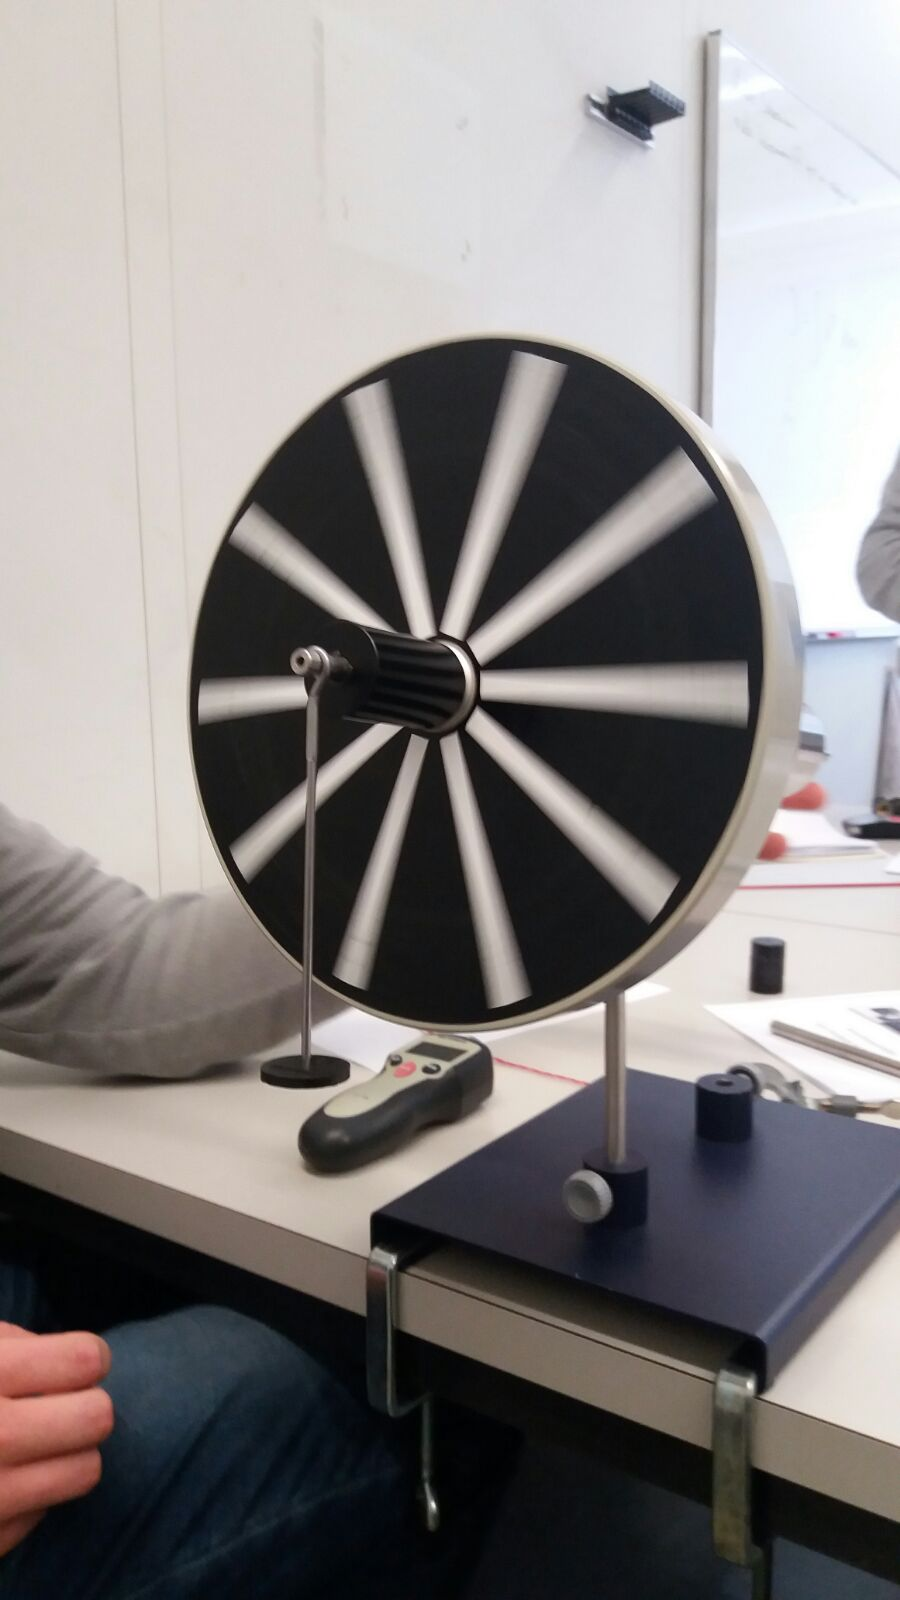
\includegraphics[scale=0.25]{aufbau.jpg}
        \captionof{figure}[]{Versuchsaufbau}
   \end{center}

\section{Versuchteil 1}
Im ersten Versuchsteil geht es um die Bestimmung des Trägheitsmoments eines Kreisels über die Bestimmung der Winkelbeschleunigung. Hierfür wird ein Faden mit einem Gewicht am Kreisel aufgehängt und aufgewickelt. Nach dem Aufwickeln wird das Gewicht auf Höhe der Tischkante losgelassen. Bis das Gewicht den Boden  berührt wird die Zeit gestoppt und die Drehzahl bestimmt.\\
\\
\section{Versuchteil 2}
Im zweiten Versuchsteil soll das Abbremsen - durch die Reibung - gemessen werden. Hierfür wird der Kreisel auf eine Drehzahl zwischen 400 und 500 Umdrehungen pro Minute gebracht. Alle 5 Sekunden wird im Zeitraum einer Minute die Drehzahl aufgezeichnet. Dies wird dreimal wiederholt.\\
\\
\section{Versuchteil 3}
In diesem Versuchteil soll das Trägheitsmoment des Kreisels über die Präzessionsfrequenz bestimmt. Hierfür muss zunächst die Arretierung entfernt werden, so dass sich der Kreisel frei drehen kann. 
Zur Bestimmung der Zeit einer halben Präzessionsumdrehung wird ein Gewicht an den Kreisel angehängt und auf eine Drehzahl von 300 bis 800 Umdrehungen pro Minute gebracht. Danach wird die Zeit einer halben Umdrehung gestoppt und die Drehzahl nach einer halben Umdrehung gemessen. Dies wird für die Gewichte von 10 g und 60 g jeweils 10 mal wiederholt.
\\
\section{Versuchteil 4}
Im letzten Versuchsteil geht es um die Bestimmung des Trägheitsmoments durch die Messung der Nutationsfrequenz. Hierfür wird der Kreisel auf eine Drehzahl zwischen 150 und 500 Umdrehungen pro Minute gebracht. Nach Loslassen des Kreisels wird dem Kreisel ein Stoß versetzt. Anschließend wird die Zeit von 5 Nutationsschwingungen und die Drehzahl nach diesen Schwingungen gemessen. 
	\pagebreak


	\chapter{Formeln}
 Der Eigendrehimpuls $\vec L$  beschreibt die Rotation eines starren Körpers um seine eigene Rotationsachse und ist definiert als:\\
    \begin{equation}
\vec L = J~\vec w
\end{equation}
Die Ableitung von $\vec L$ entspricht $ \vec M $– dem Drehmoment. Es gilt:\\
\begin{equation}
\vec{\dot{L}} = \vec{M}
\end{equation}
Für das Drehmoment $\vec M$ gilt wiederum:
\begin{equation}
\vec M = \vec r \times \vec F
\end{equation}
Das Trägheitsmoment J bezüglich einer Achse durch den Schwerpunkt wird über das Integral über die einzelnen Massenelemente bestimmt. r bezeichnet in dieser Formel den Abstand zur Drehachse.\\
\begin{equation}
J=\int_M r^2 \,dM
\end{equation}
Das Trägheitsmoment J kann auch über $\alpha$ (der Winkelbeschleunigung) und M (einem konstanten Drehmoment) bestimmt werden.\\
\begin{equation}
J=M/\alpha
\end{equation}
Zur Bestimmung unserer Werte wurde Formel (3.6) verwendet. r beschreibt den Radius, m die Masse des Körpers, g die Erdbeschleunigung, T die Periodendauer und $\omega$ der Winkelgeschwindigkeit. 
\begin{equation}
	J  = \frac{r\cdot m \cdot g \cdot T}{\omega}
\end{equation}
Die Formel zur Bestimmung der Präzessionsfrequenz $f_P$ lautet:
\begin{equation}
	f_P = \frac{r\cdot m \cdot g}{J \cdot 4 \cdot \pi ^2 \cdot f}
\end{equation}
r beschreibt den Radius, m die Masse, g dei Erdbeschleunigung, J das Trägheitsmoment und f die Erregerfrequenz.
	\pagebreak

	\chapter{Messwerte}
    
			\section{Aufgabe 1a}
            $m_1 = 0,11kg$ $r=22,5 \cdot 10^{-3} m$ \\
            \begin{center}
            	\begin{tabular}{c|cc}
                	&	Zeit $T [s]$ & Drehzahl $n [\frac{1}{min}]$ \\ \hline \hline
                    1	&	4,62	&118,6 \\
                    2	&	4,55	&114,5 \\
                    3   &	4,79	&114,6 \\
                    4   &	4,68	&117,4 \\
                    5   &	4,60	&112,9 
   		     	\end{tabular}\\
                \captionof{table}[]{Messwerte zur Aufgabe 1a}
                \end{center}
            \section{Aufgabe 1b}
             $m_2 = 0,16kg$ $r=22,5 \cdot 10^{-3} m$ \\
             \begin{center}
        	    \begin{tabular}{c|cc}
                    &	Zeit $T [s]$ & Drehzahl $n [\frac{1}{min}]$ \\ \hline \hline
                    1&3,80	&141,3\\
                    2&3,84	&128,0\\
                    3&3,86	&129,5\\
                    4&3,83	&121,6\\
                    5&3,90	&125,8 \\
                \end{tabular}\\
                 \captionof{table}[]{Messwerte zur Aufgabe 1b}
                \end{center}
			\section{Aufgabe 2}
            \begin{center}
				\begin{tabular}{c|ccc}
                    Zeit T [s] &$[\frac{1}{min}]$& $[\frac{1}{min}]$& $[\frac{1}{min}]$\\ \hline \hline
                    0	&500	&500	&500\\
                    5	&446	&454,4	&453,1\\
                    10	&401,6	&411,8	&419,6\\
                    15	&365,4	&366,5	&374,6\\
                    20	&324,7	&324,6	&337,0\\
                    25	&287,2	&287,2	&293,1\\
                    30	&254,4	&256,8	&261,4\\
                    35	&221,8	&221,1	&219,9\\
                    40	&186,7	&190,8	&192,9\\
                    45	&144,9	&149,5	&157,7\\
                    50	&112,3	&124,5	&134,9\\
                    55	&78,3	&77,2	&102,7\\
                    60	&57,8	&55,5	&63,5\\
                \end{tabular}\\
        \captionof{table}[]{Messwerte zur Aufgabe 2}
                \end{center}
            \section{Aufgabe 3a}
            $m_3 = 0,01 kg$ $l= 0,27 m $
            \begin{center}
				\begin{tabular}{cc|c}
			Drehzahl Start $[\frac{1}{min}]$&Drehzahl Ende $[\frac{1}{min}]$& $\frac{1}{2}T [s]$  \\ \hline \hline
              300	&180	&49,14 \\
              330	&204,8	&52,76 \\
              370	&213	&59,17 \\
              410	&234	&60,00 \\
              480	&267,6	&71,00 \\
              500	&277,8	&72,89 \\
              530	&288	&77,80 \\
              570	&295	&78,25 \\
              600	&322,8	&81,73 \\
              680	&335,4	&85,99
			\end{tabular}
          \captionof{table}[]{Messwerte zur Aufgabe 3a}
            \end{center}
            \section{Aufgabe 3b}
            $m_4 = 0,06 kg$ $l= 0,27 m $
            \begin{center}
            \begin{tabular}{cc|c}
            Drehzahl Start $[\frac{1}{min}]$&Drehzahl Ende $[\frac{1}{min}]$& $\frac{1}{2}T [s]$  \\ \hline \hline
            300	&216,0	&8,13\\
            340	&310,0	&8,27\\
            380	&346,2	&8,59\\
            400	&346,1	&9,19\\
            430	&388,0	&11,00\\
            480	&432,5	&12,46\\
            500	&452,1	&11,87\\
            550	&488,0	&14,00\\
            630	&557,3	&14,35\\
            700	&597,5	&16,05
            \end{tabular} \\
                 \captionof{table}[]{Messwerte zur Aufgabe 3b}
            \end{center}
			\section{Aufgabe 4}
            \begin{center}
            \begin{tabular}{cc|c}
            Drehzal Start 1/min	&Drehzahl Ende 1/min	&5*T s \\ \hline \hline
              500	&440	&5,44\\
              440	&350	&5,58\\
              470	&414	&4,86\\
              280	&248	&8,31\\
              400	&365	&5,58\\
              300	&280	&6,16\\
              360	&325	&6,55\\
              260	&225,5	&8,46\\
              230	&209,5	&9,91\\
              160	&226,6	&14,22
            \end{tabular}
            \captionof{table}[]{Messwerte zur Aufgabe 4}
            \end{center}
	\pagebreak

	\chapter{Auswertung}
		\section{Teil 1}
			Das Trägheitsmoment wird über die Winkelbeschleunigung bei zwei verschiedenen Drehmomenten berechnet. Die Mittelwerte der Messdaten sind: \\
            \begin{center}
            \begin{tabular}{c|cc}
            					&110g 	& 160g\\ \hline \hline
                Zeit [s]& 4,648 		& 3,846\\
                Drehzahl $\omega$ $[\frac{rad}{s}]$& 115,6 &  129,24 
            \end{tabular}
            \end{center}
            
            
            \begin{align*}
            	J_1 & = \frac{r\cdot m_1 \cdot g \cdot T_1}{\omega_1} \\
                & = \frac{0,225 m \cdot 0,11kg \cdot 9,81 \frac{m}{s^2} \cdot 4,648s}{115,6 \frac{rad}{s}}   \\
                & = 9,8 \cdot 10^{-3}kgm^2
            \end{align*}
           	\begin{align*}
            	J_2 & = \frac{r\cdot m_2 \cdot g \cdot T_2}{\omega_2} \\
                & =  \frac{0,225m \cdot 0,16kg \cdot 9,81 \frac{m}{s^2} \cdot 3,846 s}{129,24 \frac{rad}{s}}  \\
                & = 10,5 \cdot 10^{-3}kgm^2
            \end{align*}
            
         \pagebreak
         
         \section{Teil 2}
         	Zur Untersuchung von Reibungseffekten wird die Abklingkonstante $\gamma$ über die zeitliche Abnahme der Winkelgeschwindigkeit $\omega$ bestimmt. \\
            Die Abnahme der Winkelgeschwindigkeit wird über die Funktion 							\begin{equation}
           		\omega(t) = \omega_0 \cdot e^{- \gamma t}
            \end{equation}
            angenähert. \\
            %
            %g(x) = 500 * e**(-b*x)
            %h(x) = 500 * e**(-c*x)
            %fit f(x) "2.txt" using 1:2 via a
            \begin{gnuplot}[terminal=pdf,terminaloptions={font ",10" linewidth 3},scale=1.2]
            set  fit  errorvariables
        	set xlabel "Zeit T [s]"
            set ylabel "Winkelgeschwindigkeit w [rad/s]"
			set logscale y
            g(x) = 500*exp(-a*x+b)
            h(x) = 500*exp(-c*x+d)
            i(x) = 500*exp(-e*x+f)
            fit g(x) "2.txt" using 1:(2*pi*($2/60)) via a,b
            fit h(x) "2.txt" using 1:(2*pi*($3/60)) via c,d
            fit i(x) "2.txt" using 1:(2*pi*($4/60)) via e,f
           
			plot "2.txt" using 1:(2*pi*($2/60)) title "Durchlauf 1", "2.txt" using 1:(2*pi*($3/60)) title "Durchlauf 2", "2.txt" using 1:(2*pi*($4/60)) title "Durchlauf 3", g(x), h(x), i(x)
		\end{gnuplot}
        \captionof{figure}[]{Abbremsung des Kreisels durch Reibung}
        \ \\
        Als Abklingkonstanten ergeben sich
        \begin{align*}
       		& \gamma_1 = 25,9 \cdot 10^{-3} \frac{1}{s}\\
            & \gamma_2 = 27,1 \cdot 10^{-3} \frac{1}{s}\\
            & \gamma_3 = 27,2 \cdot 10^{-3} \frac{1}{s}
        \end{align*}

        und ihr Mittelwert $\bar{\gamma} = 26,73 \cdot 10^{-3} \frac{1}{s}$
	\pagebreak
	\section{Teil 3}
  	Der konstante Faktor $\frac{t_p}{f}$, der mithilfe der Messwerte gemittelt werden kann.
    
    \begin{equation}
    	J = \frac{r\cdot m \cdot g}{4\pi^2} \frac{T_p}{f}
        \label{Formelfuerk1_1}
    \end{equation}
    \begin{equation}
    	\frac{t_p}{f} = k \longrightarrow T_p = k \cdot f 
        \label{Formelfuerk1_2}
    \end{equation}
    \begin{gnuplot}[terminal=pdf,terminaloptions={font ",10" linewidth 3},scale=1.2]
    		set  fit errorvariables
        	set xlabel "Erregerfrequenz f [Hz]"
            set ylabel "Präzzesionsdauer Tp [s]"
			set yrange [0:200]
            f(x) = a*x + b
            g(x) = c*x + d
            fit  f(x) "3a.csv" using (($1+$2)/120):(2*$3):($4/60)  via a,b
            fmax(x)=(a+a_err)*x + b-b_err
            fmin(x)=(a-a_err)*x + b+b_err
            fit  g(x) "3b.csv" using (($1+$2)/120):(2*$3):($4/60)  via c,d
            gmax(x)=(c+c_err)*x + d-d_err
            gmin(x)=(c-c_err)*x + d+d_err
            
        
 
			plot "3a.csv" using (($1+$2)/120):(2*$3):(2*$6):($4/60) with xyerrorbars title "10g", "3b.csv" using (($1+$2)/120):(2*$3):(2*$6):($4/60) with xyerrorbars title "60g" , f(x), g(x), fmax(x),fmin(x),gmax(x),gmin(x)
		\end{gnuplot}
        \captionof{figure}[]{Analyse der Abhängigkeit von Erreger- und Präzessionfrequenz}
        \ \\
        Für 10g gilt $k_1 = 17,3146 \cdot 10^{-3} ~ s^2$ und für 60g gilt $k_2 = 2,7097 ~ s^2$

    
    \begin{align*}
    	J_1 & = \frac{r\cdot m \cdot g}{4\pi^2} \cdot k_1 \\
        	& = \frac{0,27 m \cdot 0,01kg \cdot 9,81 \frac{m}{s^2}}{4\pi^2} \cdot 17,3146 s^2 \\
            & = 11,6 \cdot 10^{-3} kgm^2
    \end{align*}
    \begin{align*}
    	J_2 & = \frac{r\cdot m \cdot g}{4\pi^2} \cdot k_2 \\
        	& = \frac{0,27 m \cdot 0,06kg \cdot 9,81 \frac{m}{s^2}}{4\pi^2} \cdot 2,7097 s^2 \\
            & = 10,9 \cdot 10^{-3}kgm^2
    \end{align*}
    \pagebreak
    	\section{Teil 4}
        	Den linearen Zusammenhang zwischen Kreiselfrequenz und Nutationsfrequenz erkennt man an der Ausgleichsgerade. \\
        	\begin{gnuplot}[terminal=pdf,terminaloptions={font ",10" linewidth 3},scale=1.2]
            set key  bottom
            set fit errorvariables
        	set xlabel "Erregerfrequenz f [Hz]"
            set ylabel "Nutationsfrequenz f_n [hz]"
			f(x) = a*x + b
           
            fit f(x) "4.csv" using (($1+$2)/120):(5/$3) via a,b
            fmax(x)=(a+a_err)*x + b-b_err
            fmin(x)=(a-a_err)*x + b+b_err
			plot "4.csv" using (($1+$2)/120):(5/$3):($4/60):($6/5) with xyerrorbars title "60g", f(x), fmin(x),fmax(x)
		\end{gnuplot}
        \captionof{figure}[]{Analyse der Abhängigkeit von Erreger- und Nutationsfrequenz}
	\chapter{Fehlerrechnung}
    	\section{Fehler für J}
        \begin{itemize}
        \item $\Delta T = 0,5 s$
        \item $\Delta n = 10 \frac{1}{min} $
        \item $\Delta \omega = 2 \pi \cdot \frac{\Delta n}{60\frac{s}{min}}$ = $\frac{2}{6} \pi \approx 1,05 \frac{rad}{s}$
        \end{itemize}
        Berechnet wurde J mithilfe der Formel:
        \begin{align*}
            	J & = \frac{r\cdot m_1 \cdot g \cdot T}{\omega}
            \end{align*}
    	\begin{align*}
    		\Delta J_1 & = |\frac{\partial J}{\partial x_i}| \Delta x_i \\
            		& = |\frac{\partial J}{\partial \omega}| \Delta \omega + |\frac{\partial J}{\partial T}| \Delta T \\ 
                    & = |-\frac{r \cdot m_1 \cdot g \cdot T}{\omega^2}| \Delta \omega + |\frac{r\cdot m_1 \cdot g}{\omega}| \Delta T \\ 
                     & = |-\frac{0,225 m \cdot 0,11kg \cdot 9,81 \frac{m}{s^2} \cdot 4,648 s}{(115,6 \frac{rad}{s})^2}| 1,05 \frac{rad}{s} + |\frac{0,225m \cdot 0,11kg \cdot 9,81 \frac{m}{s^2}}{115,6 \frac{rad}{s}}| 0,5 s \\ 
                     & = 1,59 \cdot 10^{-3} kgm^2
    	\end{align*}
        Analog für $\Delta J_2 = 1,6 \cdot 10^{-3} kgm^2$  
        \section{Teil 2}
        	Der Fit mit GnuPlot ergab für die Fehlergeraden die Abweichungen von der Steigung: \\
            \begin{center}
            
            
            \begin{tabular}{c|c}
             & $[kgm^2]$ \\ \hline
             $\Delta\gamma_1$ & $1,4 \cdot 10^{-3}$ \\
             $\Delta\gamma_2$ & $1,6 \cdot 10^{-3}$\\
             $\Delta\gamma_3$ & $1,7 \cdot 10^{-3}$
            \end{tabular} 
            \end{center}
            und der Mittelwert $\Delta\bar{\gamma} = 1,57 \cdot 10^{-3} kgm^2$.
            
       \section{Teil 3}
       		Der Fit zur Bestimmung der Konstante k in Formel \ref{Formelfuerk1_1} mit GnuPlot ergab folgende Fehler:
       		\begin{center}
       		
       		\begin{tabular}{c|c}
             		&	$[s^2]$\\ \hline
       			$\Delta k_1$ & $0,9119$ \\
                $\Delta k_2$ & $0,2394$
       		\end{tabular}
            
       		\end{center}
            Das Trägheitsmoment wurde berechnet über
           $ J  = \frac{r\cdot m \cdot g}{4\pi^2} \cdot k_1 $
           \begin{align*}
           		\Delta J_1 & = |\frac{r\cdot m_1 \cdot g}{4\pi^2}| \Delta k_1\\
                & = |\frac{0,27 m\cdot 0,01 kg \cdot 9,81 \frac{m}{s^2}}{4\pi^2}| 0,9119 s^2 \\
                & = 0,6 \cdot 10^{-3} kgm^2
           \end{align*}
           		Analog dazu $J_2 = 1,0 \cdot 10^{-3}kgm^2$
	\pagebreak

	\chapter{Zusammenfassung}
    Das Trägheitsmoment der einzelnen Aufgaben mit Fehler beträgt.
    \begin{center}
    \begin{tabular}{c|c}
    	Teil 1 &  $[kgm^2]$\\ \hline \hline
        $J_1$ & $(9,8\pm 1,59) \cdot 10^{-3}$\\
        $J_2$ & $(10,5\pm 1,6) \cdot 10^{-3}$\\ \hline
        Teil 3 & $[kgm^2]$\\ \hline \hline
        $J_1$ & $(11,6\pm 0,6) \cdot 10^{-3}$\\
        $J_2$ & $(10,9\pm 1,0) \cdot 10^{-3}$\\
        
    \end{tabular}
    \end{center}
   	Für die Abklingkonstante gilt $\gamma = (26,73\pm 1,57) \cdot 10^{-3} \frac{1}{s}$
    Gründe für die Fehler sind:
    \begin{enumerate}
    \item Ablesegenauigkeiten, wann eine halbe Umdrehung (Präzession) oder wann 5 Umdrehungen (Nutation) vorbei sind.
    \item Messgenauigkeit beim Stoppen der Zeit durch Ungenauigkeit der Stoppuhr und Reaktionszeit bis zum drücken des Stoppknopfes.
    \item Ungenauigkeit beim Drehzahlmessen, da auch der Drehzahmesser nur eine gewisse Genauigkeit hat. 
    \end{enumerate}
 
    
	\pagebreak

	\chapter{Anhang}
    \begin{center}
    		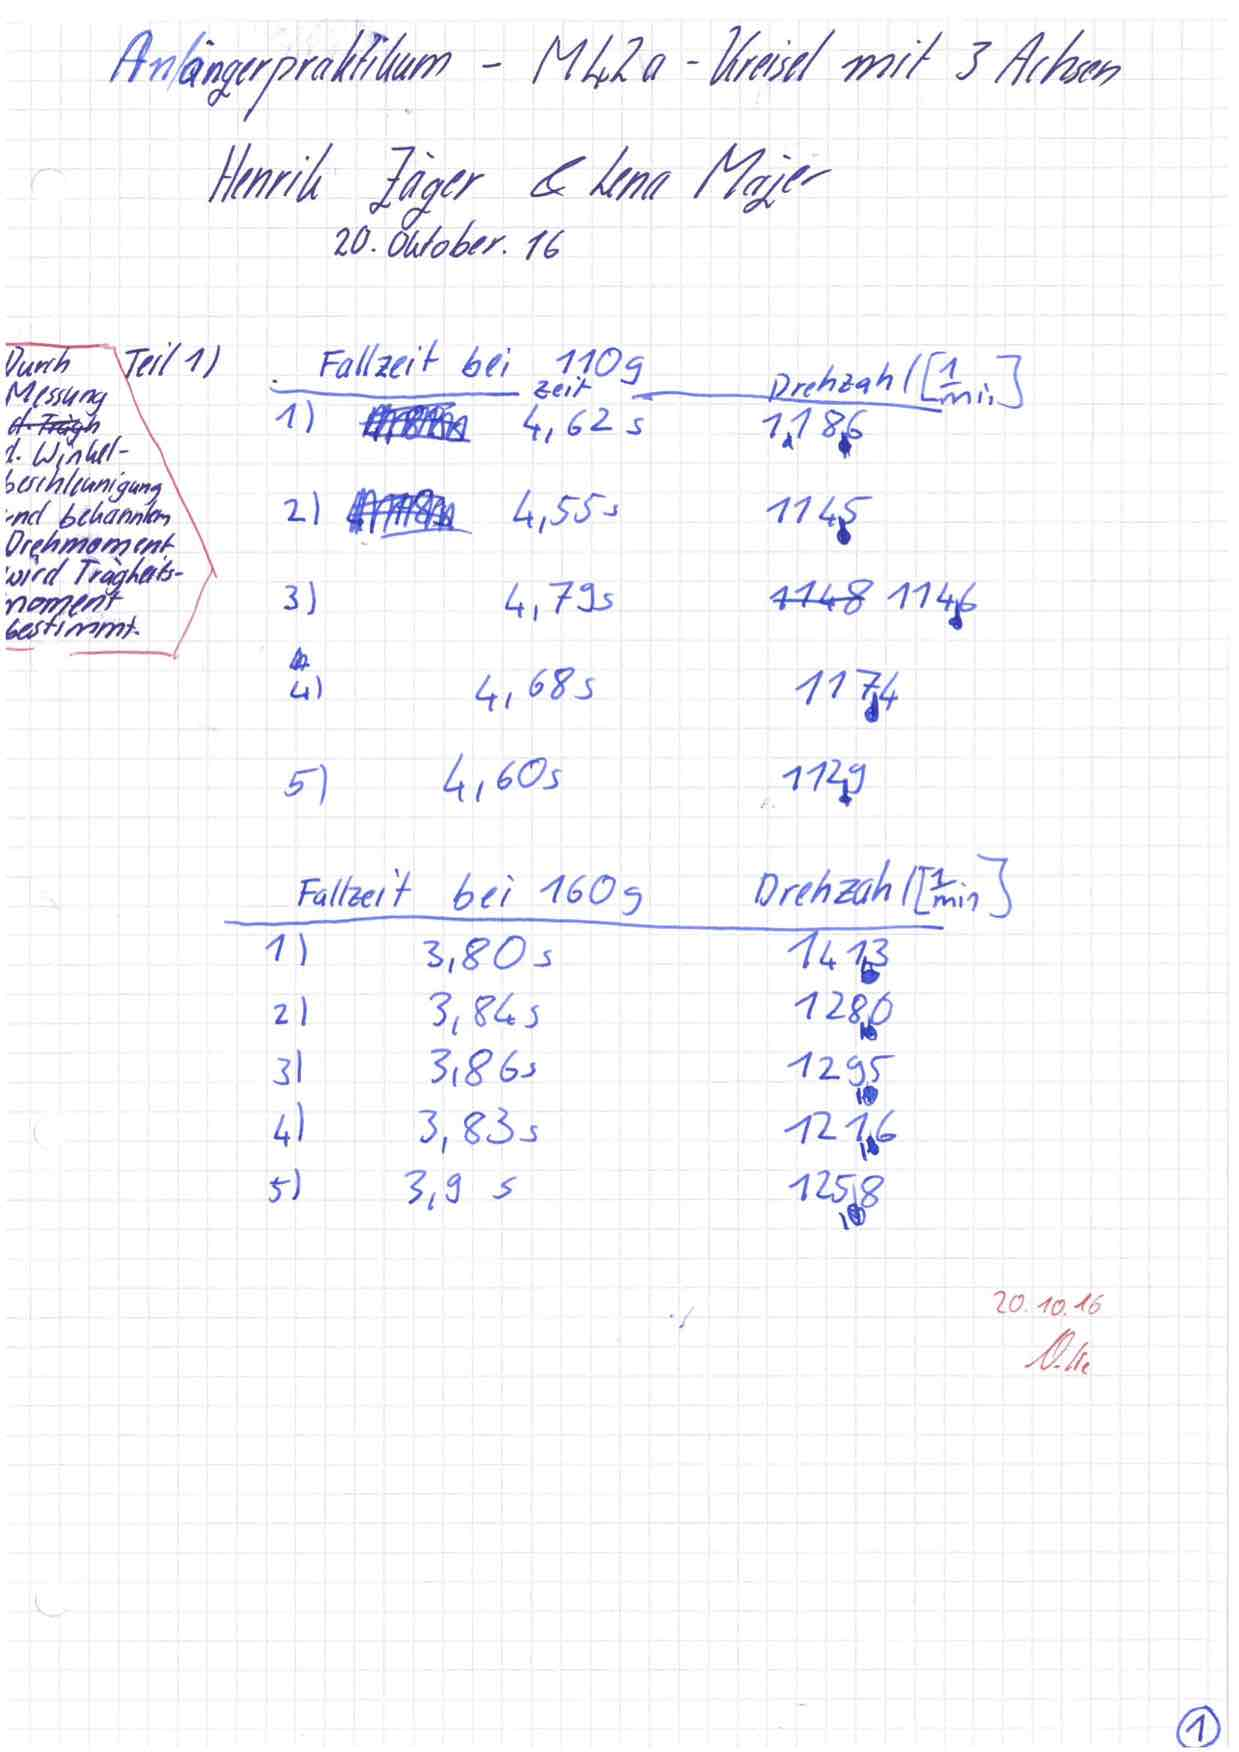
\includegraphics[scale=0.32]{1.jpg}
    	\end{center}
    	\captionof{figure}[Seite 1]{Messprotokoll Seite 1}
    	\pagebreak
    	
        \begin{center}
    		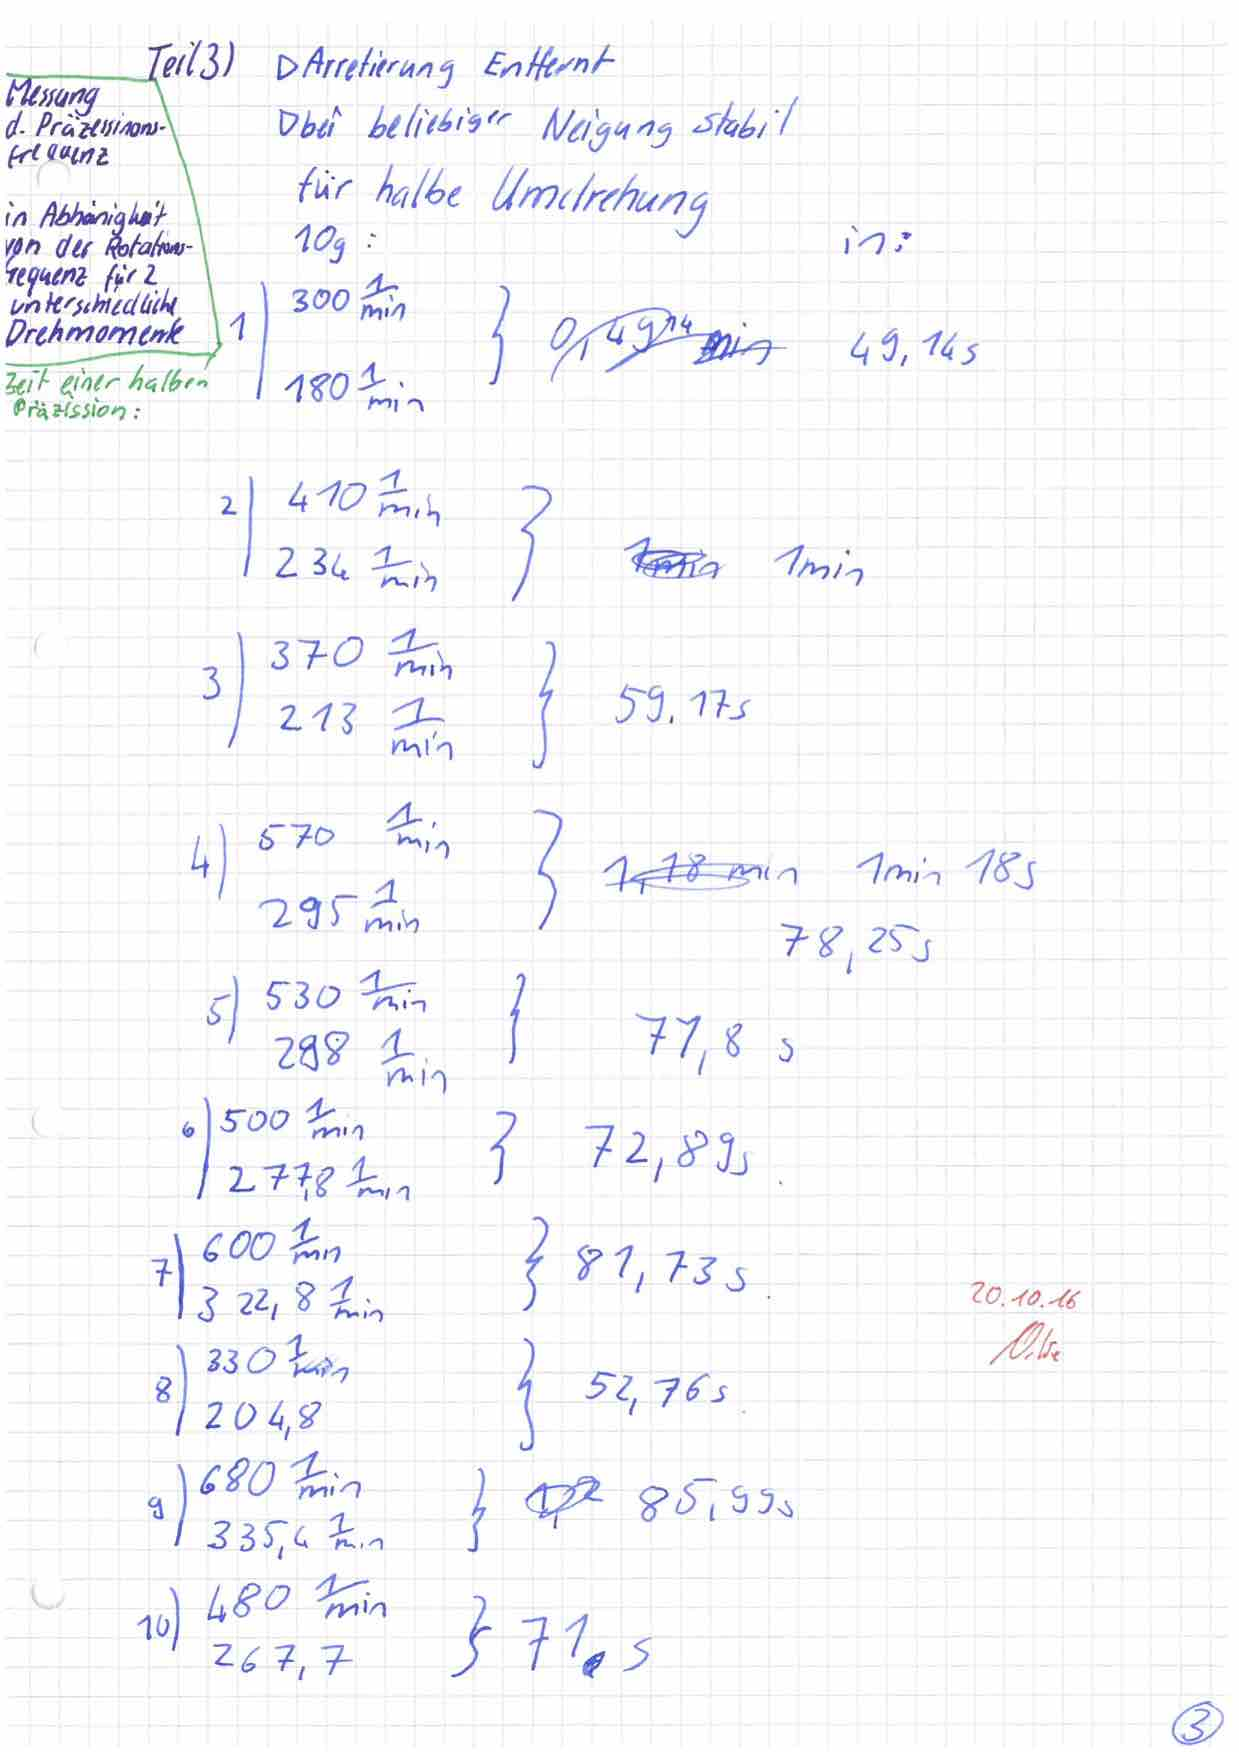
\includegraphics[scale=0.32]{2.jpg}
    	\end{center}
    	\captionof{figure}[Seite 2]{Messprotokoll Seite 2}
    	\pagebreak
    	
        \begin{center}
   		 	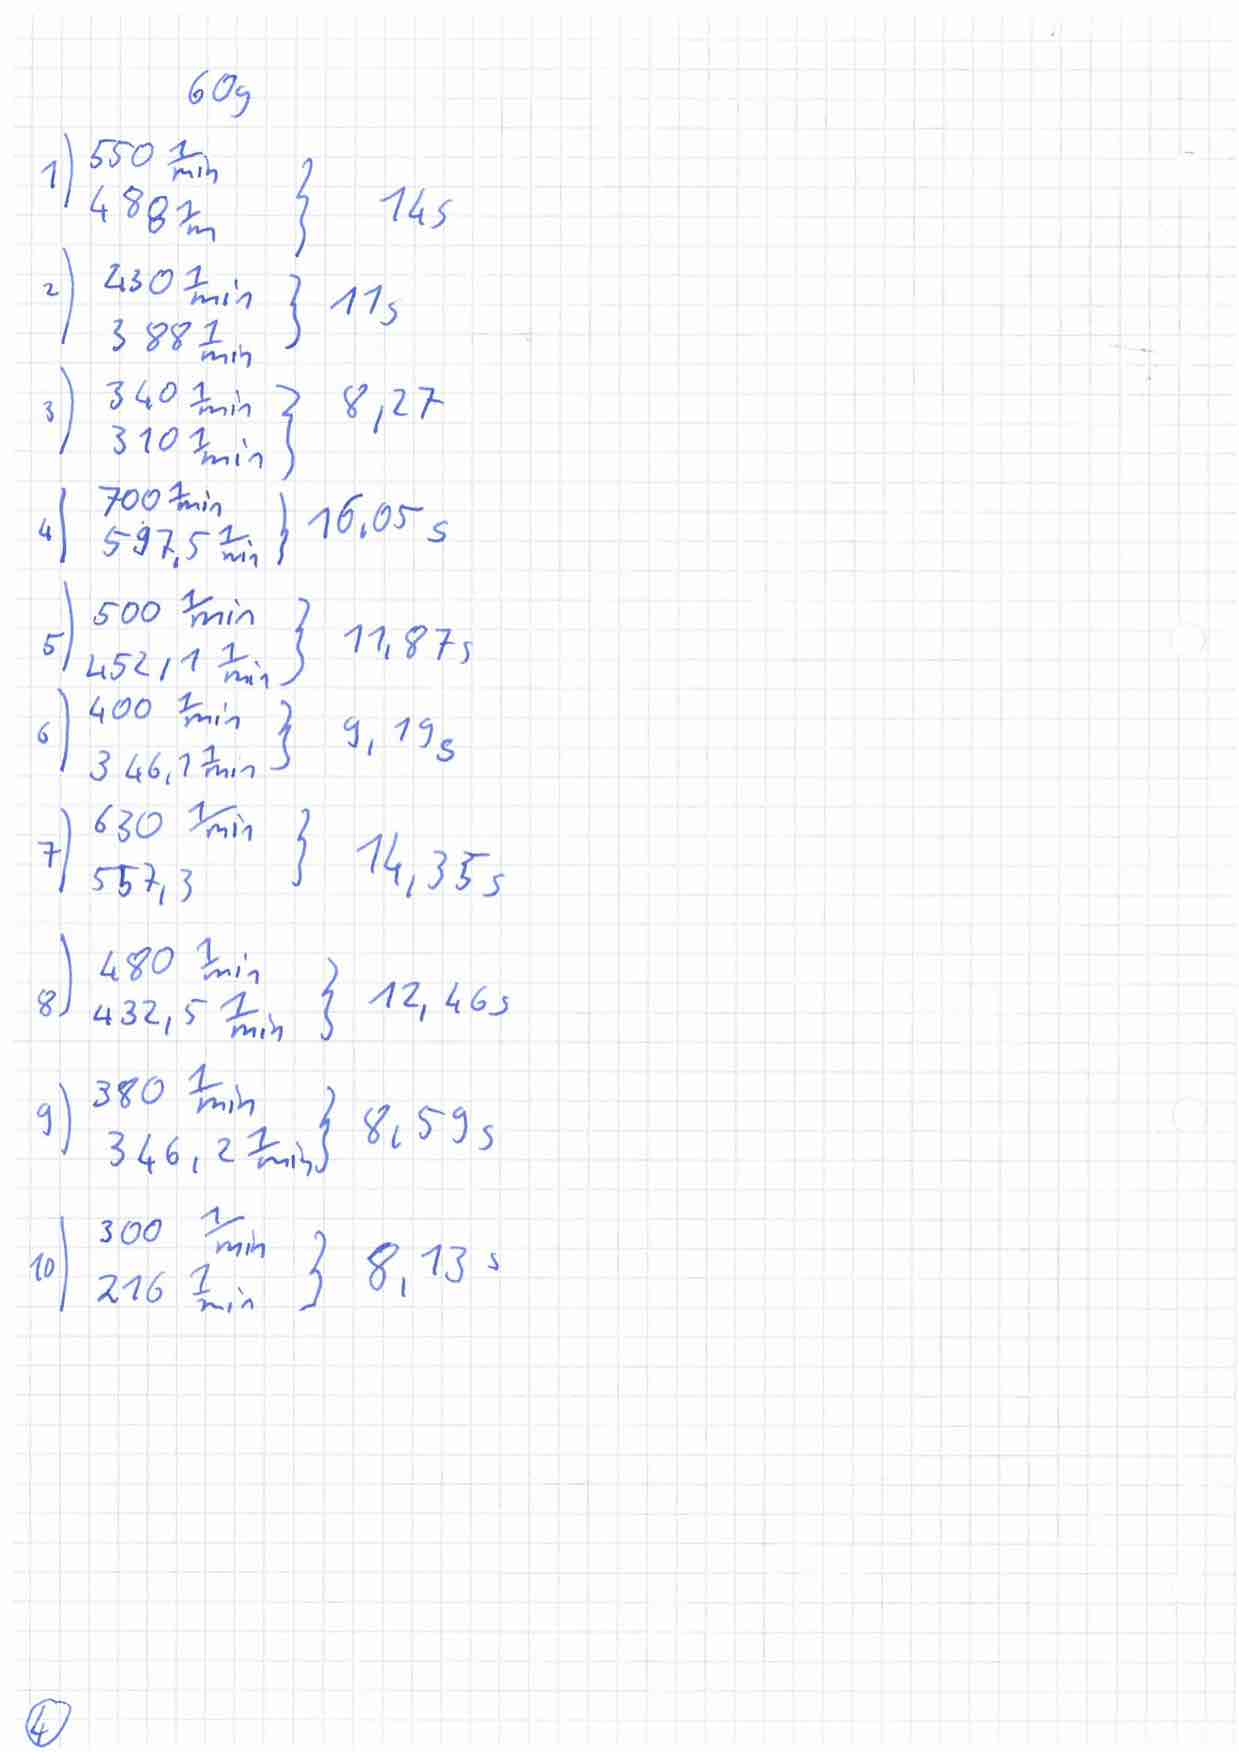
\includegraphics[scale=0.32]{3.jpg}
   	 	\end{center}
    	\captionof{figure}[Seite 3]{Messprotokoll Seite 3}
    	\pagebreak
    	
        \begin{center}
    		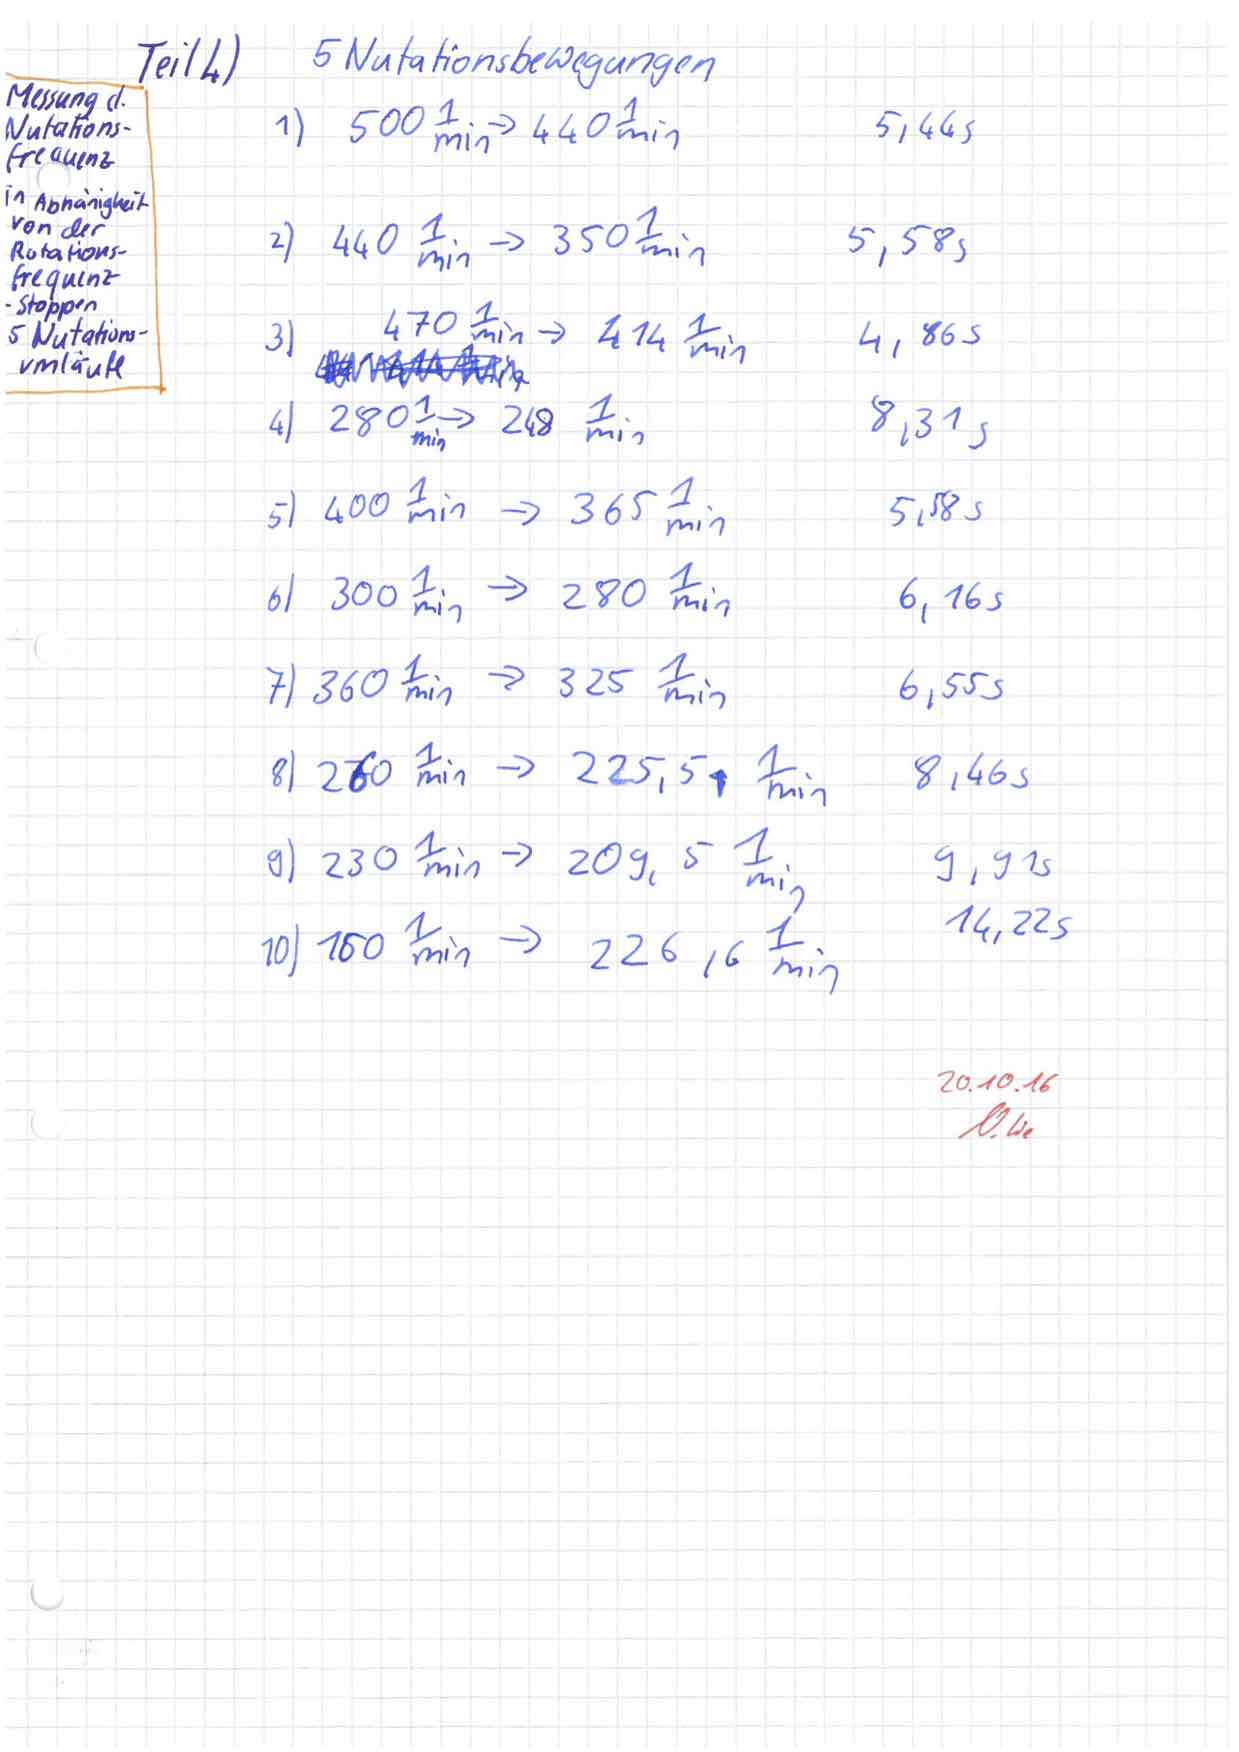
\includegraphics[scale=0.32]{4.jpg}
    	\end{center}
    	\captionof{figure}[Seite 4]{Messprotokoll Seite 4}
    	\pagebreak
    	
        \begin{center}
    		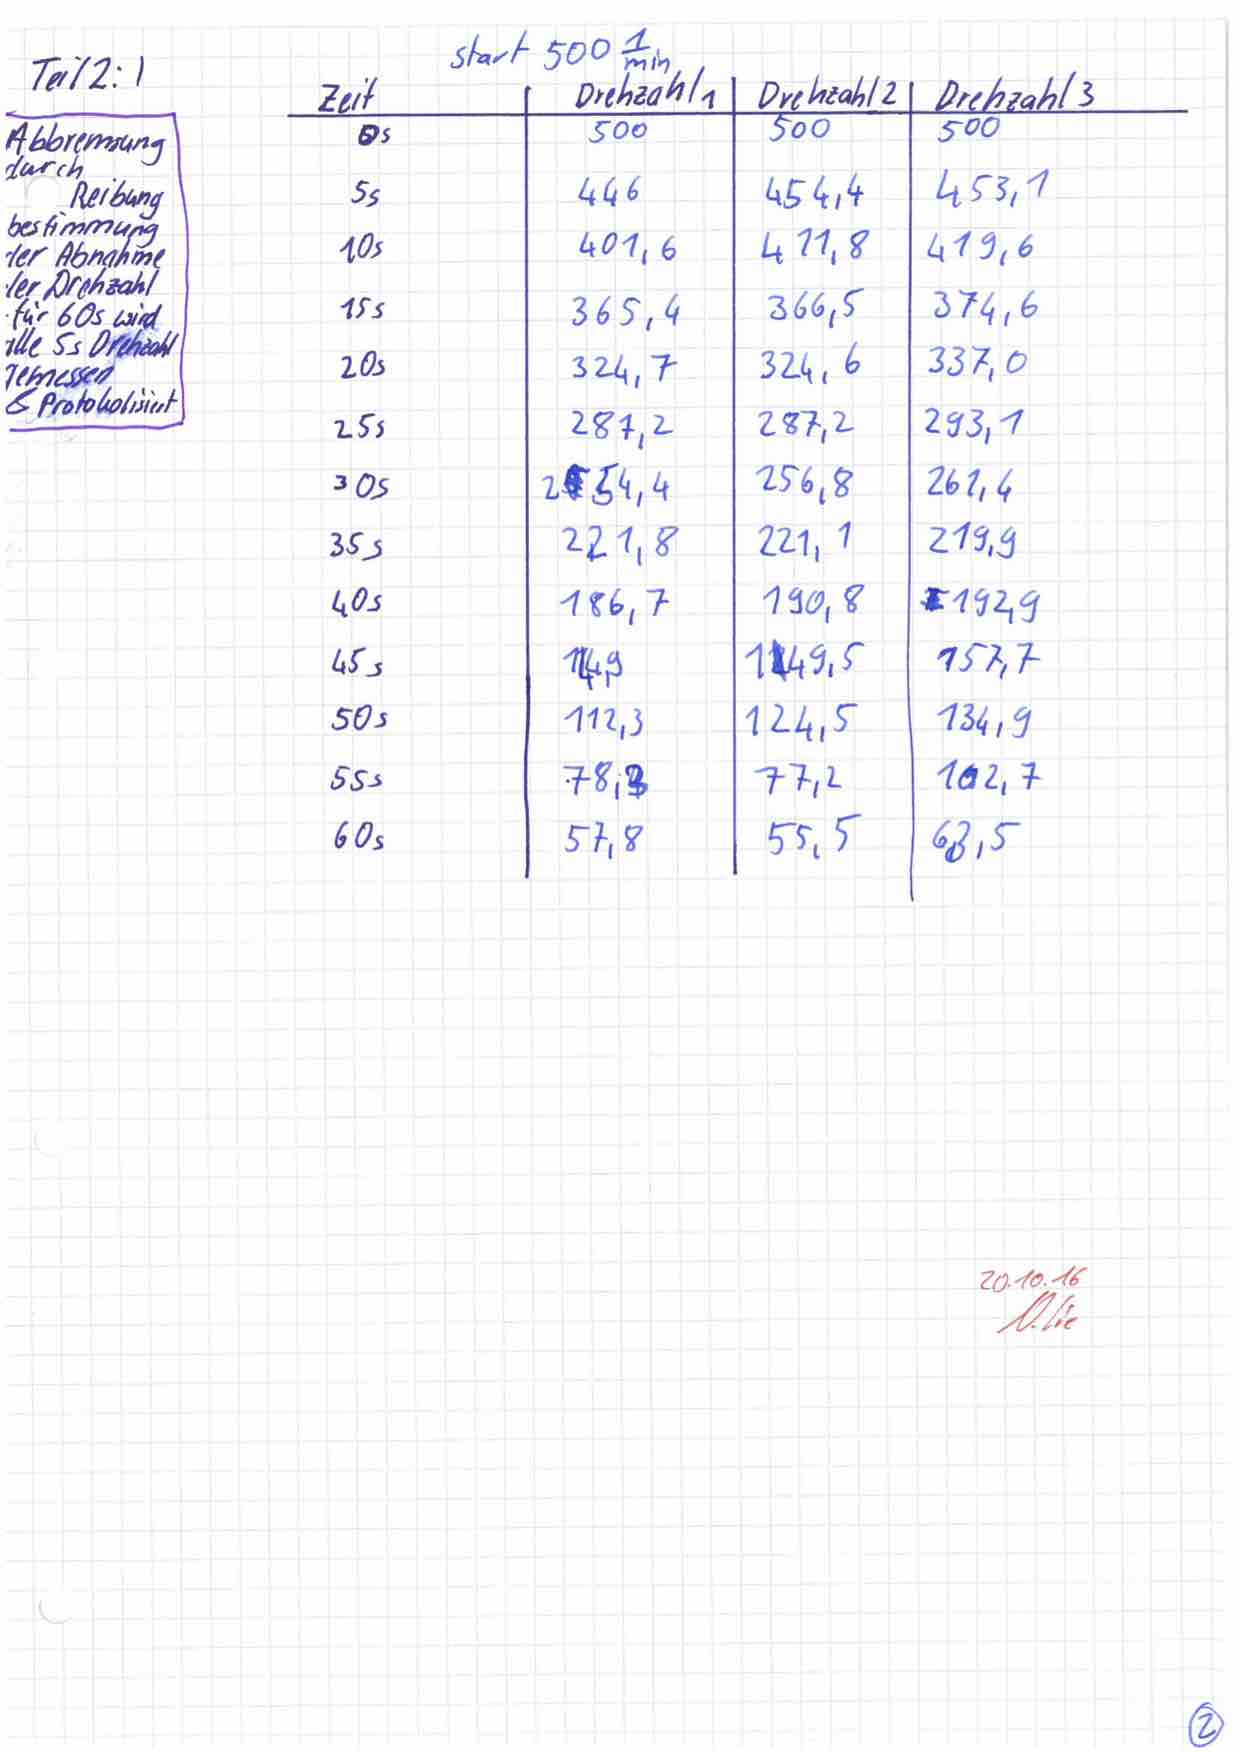
\includegraphics[scale=0.32]{5.jpg}
    	\end{center}
    	\captionof{figure}[Seite 5]{Messprotokoll Seite 5}
    	
	\pagebreak




\end{document}